\documentclass[12pt]{report}\usepackage[]{graphicx}\usepackage[dvipsnames]{xcolor}
% maxwidth is the original width if it is less than linewidth
% otherwise use linewidth (to make sure the graphics do not exceed the margin)
\makeatletter
\def\maxwidth{ %
  \ifdim\Gin@nat@width>\linewidth
    \linewidth
  \else
    \Gin@nat@width
  \fi
}
\makeatother

\definecolor{fgcolor}{rgb}{0.345, 0.345, 0.345}
\newcommand{\hlnum}[1]{\textcolor[rgb]{0.686,0.059,0.569}{#1}}%
\newcommand{\hlstr}[1]{\textcolor[rgb]{0.192,0.494,0.8}{#1}}%
\newcommand{\hlcom}[1]{\textcolor[rgb]{0.678,0.584,0.686}{\textit{#1}}}%
\newcommand{\hlopt}[1]{\textcolor[rgb]{0,0,0}{#1}}%
\newcommand{\hlstd}[1]{\textcolor[rgb]{0.345,0.345,0.345}{#1}}%
\newcommand{\hlkwa}[1]{\textcolor[rgb]{0.161,0.373,0.58}{\textbf{#1}}}%
\newcommand{\hlkwb}[1]{\textcolor[rgb]{0.69,0.353,0.396}{#1}}%
\newcommand{\hlkwc}[1]{\textcolor[rgb]{0.333,0.667,0.333}{#1}}%
\newcommand{\hlkwd}[1]{\textcolor[rgb]{0.737,0.353,0.396}{\textbf{#1}}}%
\let\hlipl\hlkwb

\usepackage{framed}
\makeatletter
\newenvironment{kframe}{%
 \def\at@end@of@kframe{}%
 \ifinner\ifhmode%
  \def\at@end@of@kframe{\end{minipage}}%
  \begin{minipage}{\columnwidth}%
 \fi\fi%
 \def\FrameCommand##1{\hskip\@totalleftmargin \hskip-\fboxsep
 \colorbox{shadecolor}{##1}\hskip-\fboxsep
     % There is no \\@totalrightmargin, so:
     \hskip-\linewidth \hskip-\@totalleftmargin \hskip\columnwidth}%
 \MakeFramed {\advance\hsize-\width
   \@totalleftmargin\z@ \linewidth\hsize
   \@setminipage}}%
 {\par\unskip\endMakeFramed%
 \at@end@of@kframe}
\makeatother

\definecolor{shadecolor}{rgb}{.97, .97, .97}
\definecolor{messagecolor}{rgb}{0, 0, 0}
\definecolor{warningcolor}{rgb}{1, 0, 1}
\definecolor{errorcolor}{rgb}{1, 0, 0}
\newenvironment{knitrout}{}{} % an empty environment to be redefined in TeX

\usepackage{alltt}

\usepackage[spanish]{babel}
\usepackage[margin = 2.54cm]{geometry}
\usepackage[dvipsnames]{xcolor}
\usepackage[most]{tcolorbox}
\usepackage{amssymb, amsthm, array, cancel, enumitem, fancyhdr, float, graphicx, hyperref, hologo, listings, mathtools, qtree, tikz, tikz-cd}
\usepackage[spanish, noabbrev]{cleveref}

\pagestyle{fancy}
\lhead{\footnotesize \leftmark}
\rhead{\footnotesize \rightmark}

\lstdefinestyle{estilo_pablo}{
	basicstyle = \ttfamily\footnotesize, 
	tabsize = 2, 
	commentstyle = \color{gray}, 
	keywordstyle = \color{cyan}, 
	stringstyle = \color{purple}, 
	tabsize = 1, 
	frame = tb, 
	breaklines = true, 
	showstringspaces = false, 
	numbers = left, 
	numberstyle = \footnotesize\color{gray}, 
	stepnumber = 1, 
	captionpos = b
}

\crefname{listing}{Código}{Códigos}
\crefname{section}{Sección}{Secciones}

\title{
	\huge
	\noindent\textbf{Fundamentos de la Ciencia de Datos}\\
	
	{\Large \textit{Práctica 2}}
	\vspace{1cm}
	
	\huge
	Grado en Ingeniería Informática\\
	Universidad de Alcalá\\
	
	\vspace{1cm}
	
	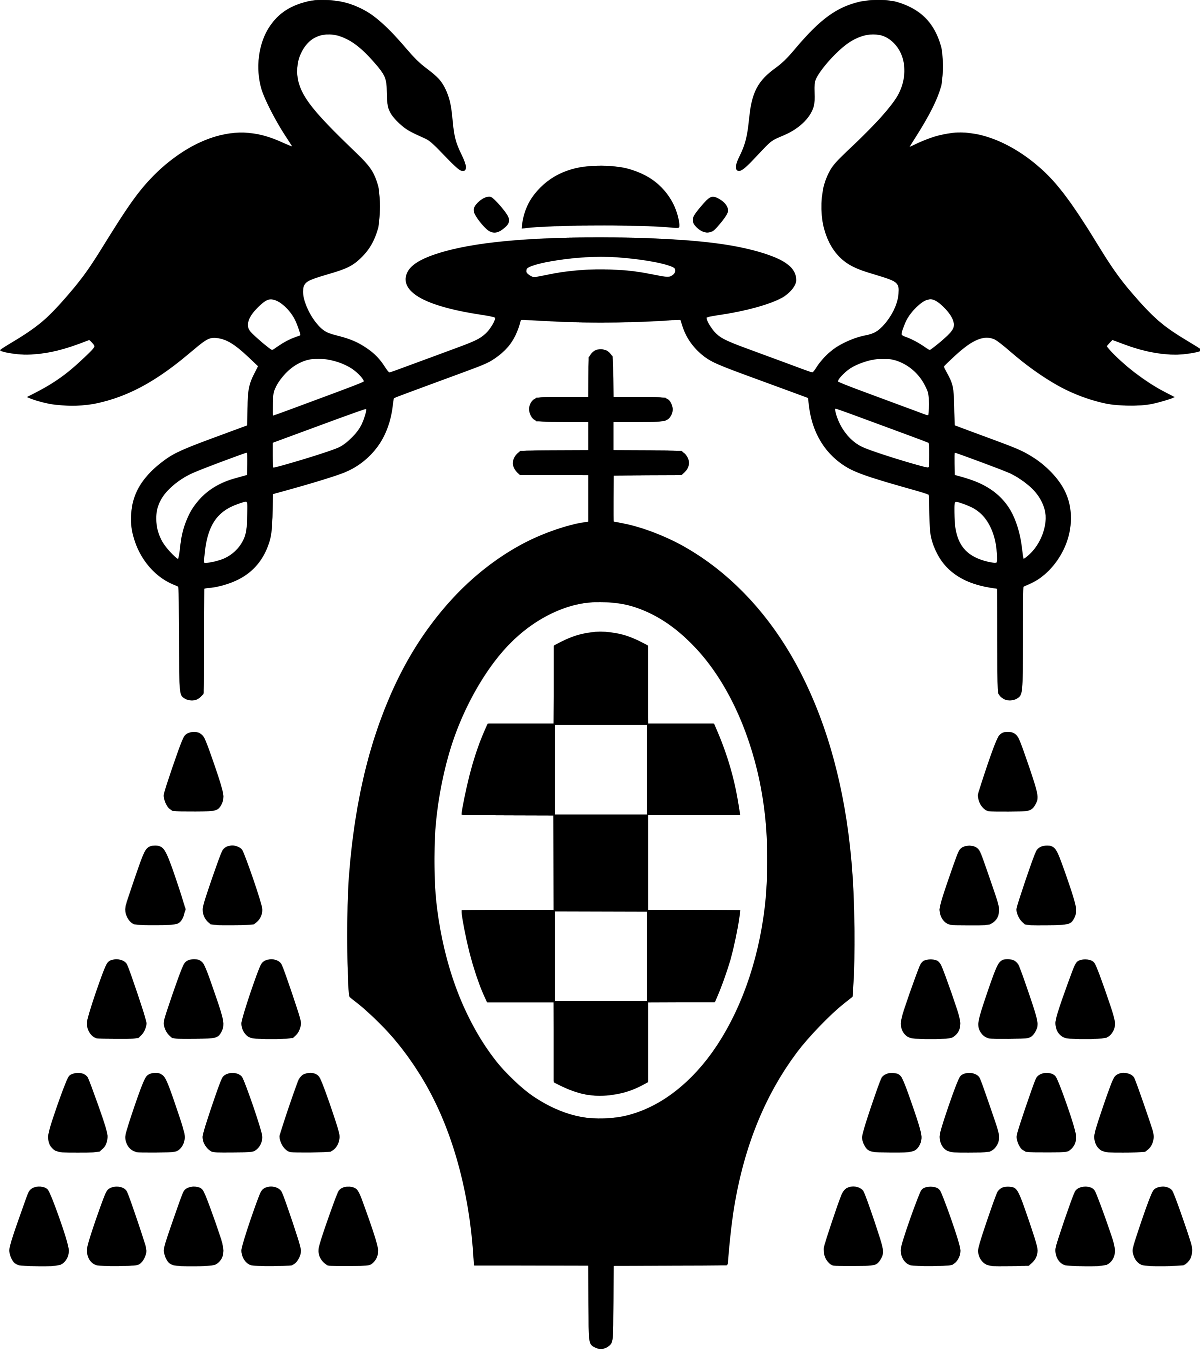
\includegraphics[scale = 0.075]{img/logo}
}

\author{
	Grupo 9\\\\
	Pablo García García\\
	Abel López Martínez\\
	Álvaro Jesús Martínez Parra\\
	Raúl Moratilla Núñez
}

\date{
	\large{\today}
}

\hypersetup{
	pdftitle = {Práctica 2}, 
	pdfauthor = {Pablo García García, Abel López Martínez, Álvaro Jesús Martínez Parra, Raúl Moratilla Núñez}, 
	pdfsubject = {Fundamentos de la Ciencia de Datos}, 
	pdfcenterwindow, 
	pdfnewwindow = true, 
	pdfkeywords = {Entrega de la PL2 de laboratorio correspondiente al Curso 2023-2024}, 
	bookmarksopen = true 
}

\newtheorem{exercise}{Ejercicio}[section]
\newtheorem{observation}{Observación}[section]
\newtcbtheorem[number within = section, Crefname = {Teorema}{Teorema}]{teorema}{Teorema}{fonttitle = \bfseries}{th}
\newtcbtheorem[number within = section, Crefname = {Definición}{Definición}]{definicion}{Definición}{fonttitle = \bfseries}{df}

\newcommand{\dt}{\text{dist}}
\newcommand{\ds}{\text{dens}}
\newcommand{\drm}{\text{drm}}

\newcommand{\rojo}[1]{\textcolor{Red}{#1}}
\IfFileExists{upquote.sty}{\usepackage{upquote}}{}
\begin{document}
	
	\renewcommand{\chaptername}{Parte}
	\renewcommand{\lstlistingname}{Código}
	\maketitle \thispagestyle{empty}
	
	\newpage
	
	\setcounter{tocdepth}{3}
	\tableofcontents
	
	\chapter*{Introducción}\addcontentsline{toc}{chapter}{Introducción}\pagestyle{plain}
	
	\chapter{Ejercicios guiados}\pagestyle{fancy}
	
	En esta primera parte de la práctica, se repetirán los ejercicios explicados y realizados por el profesor en las clases de laboratorio, utilizando los mismos procedimientos vistos y plasmándolos en este documento.
	
	\section{Clasificación No Supervisada con K-Means}
	
	\begin{exercise}
		El primer conjunto de datos, que se empleará para realizar el análisis de clasificación no supervisada con KMeans, estará formado por las siguientes 8 calificaciones de estudiantes: 1. \{4, 4\}; 2. \{3, 5\}; 3. \{1, 2\}; 4. \{5, 5\}; 5.\{0, 1\}; 6. \{2, 2\}; 7. \{4, 5\}; 8. \{2, 1\}, donde las características de las calificaciones son: \{Teoría, Laboratorio\}.
	\end{exercise}
	
	\section{Clasificación No Supervisada con CJA}
	
	\begin{exercise}
		El segundo conjunto de datos, que se empleará para realizar el análisis de clasificación no supervisada con Clusterización Jerárquica Aglomerativa, estará formado por 6 calificaciones de estudiantes: 1. \{0.89, 2.94\}; 2.\{4.36, 5.21\}; 3. \{3.75, 1.12\}; 4. \{6.25, 3.14\}; 5. \{4.1, 1.8\}; 6. \{3.9, 4.27\}.
	\end{exercise}
	
	\section{Clasificación Supervisada con Árboles de Decisión}
	
	\begin{exercise}
		El tercer conjunto de datos, que se empleará para realizar el análisis de clasificación supervisada utilizando árboles de decisión, estará formado por las siguientes 9 calificaciones de estudiantes: 1. \{A, A, B, Ap\}; 2. \{A, B, D, Ss\}; 3. \{D, D, C, Ss\}; 4. \{D, D, A, Ss\}; 5. \{B, C, B, Ss\}; 6. \{C, B, B, Ap\}; 7. \{B, B, A, Ap\}; 8. \{C, D, C, Ss\}; 9. \{B, A, C,
		Ss\}, donde las características de las calificaciones son: \{Teoría, Laboratorio, Prácticas, Calificación Global).
	\end{exercise}
	
	\newpage
	
	\section{Clasificación Supervisada con Regresión}
	
	\begin{exercise}
		El cuarto conjunto de datos, que se empleará para realizar el análisis de clasificación supervisada utilizando regresión, estará formado por los siguientes 4 radios ecuatoriales y densidades de los planetas interiores:
		\{Mercurio, 2.4, 5.4; Venus, 6.1, 5.2; Tierra, 6.4, 5.5; Marte, 3.4, 3.9\}.
	\end{exercise}
	
	Para empezar este ejercicio se deberán introducir los datos expuestos en el enunciado en un archivo de texto (\texttt{.txt}), con el fin de ser posteriormente leídos. La inserción de los datos en este fichero se hará atendiendo a las normas relacionadas con este tipo de archivos que ya se vieron en la primera práctica. Estas normas son las siguientes:
	
	\begin{itemize}
		\item Existirá una tabulación entre dato y dato. 
		\item La primera columna numera las filas, y en la primera fila se introduce un espacio y el nombre de las variables. 
		\item Se introducirá un salto de línea en la última fila. 
		\item Para los números decimales se utilizarán puntos. 
		\item Al escribir nombres, no se deberán introducir espacios. 
	\end{itemize}
	
	Obedeciendo estas normas, se copian los datos en un fichero llamado \texttt{planetas.txt}, y se carga en R de la siguiente manera:
	
\begin{knitrout}
\definecolor{shadecolor}{rgb}{0.969, 0.969, 0.969}\color{fgcolor}\begin{kframe}
\begin{alltt}
\hlstd{(muestra} \hlkwb{=} \hlkwd{read.table}\hlstd{(}\hlstr{"data/planetas.txt"}\hlstd{))}
\end{alltt}
\begin{verbatim}
##      R   D
## 1. 2.4 5.4
## 2. 6.1 5.2
## 3. 6.4 5.5
## 4. 3.4 3.9
\end{verbatim}
\end{kframe}
\end{knitrout}
	
	Una vez se tienen los datos en R, se procede a hacer uso de la función \texttt{lm} contenida en los paquetes básicos (concretamente en el paquete \texttt{stats}). Esta función recibe dos parámetros. El primero de ellos es la fórmula en donde se va a decir en función de qué parámetro se quiere otro parámetro. En este caso se tiene la columna \texttt{R} que representa el radio y la columna \texttt{D} que representa la densidad. Como se quiere la densidad en función del radio, el primer parámetro tendrá que ser formula=D$\sim$R. Se indica de esta forma que se pretende obtener la columna \texttt{D} en función de la columna \texttt{R}; o lo que es lo mismo, la densidad en función del radio.
	
	El segundo parámetro que entra a la función es la estructura que contiene los datos que se pretenden estudiar. En este caso, el parámetro \texttt{data} será la variable \texttt{muestra}, confeccionada previamente.
	
	Con los parámetros de la función \texttt{lm} claros, se invoca a la misma de la siguiente forma:
	
\begin{knitrout}
\definecolor{shadecolor}{rgb}{0.969, 0.969, 0.969}\color{fgcolor}\begin{kframe}
\begin{alltt}
\hlstd{(regresion}\hlkwb{=}\hlkwd{lm}\hlstd{(D}\hlopt{~}\hlstd{R,} \hlkwc{data}\hlstd{=muestra))}
\end{alltt}
\begin{verbatim}
## 
## Call:
## lm(formula = D ~ R, data = muestra)
## 
## Coefficients:
## (Intercept)            R  
##      4.3624       0.1394
\end{verbatim}
\end{kframe}
\end{knitrout}
	
	En la salida de la función se observan los coeficientes que conforman la recta de regresión que mejor se adapta a los datos introducidos. El método de obtención o ajuste de la función es el de mínimos cuadrados, pudiendo comprobar que el resultado es el mismo que el que se ha visto en clase. En este método, los coeficientes se calculan de la siguiente forma, siendo $x$ el radio e $y$ la densidad:
	
	\begin{center}
		$b = \frac{s_{xy}}{s^{2}_x}$;
		$a = \overline{y} -b\overline{x}$
	\end{center}
	 
	 La salida proporciona directamente los valores de a y b, siendo estos el primero y el segundo respectivamente. Con estos valores se puede decir que la densidad de un planeta se puede sacar atendiendo a la siguiente fórmula:
	 
	 \begin{center}
	 	$D = 4.3624 + 0.1394R$
	 \end{center}
	 
	 Con el comando \texttt{summary} aplicado a la regresión que se acaba de hacer se pueden ver parámetros que detallan esta recta de regresión con respecto a los datos.
	 
\begin{knitrout}
\definecolor{shadecolor}{rgb}{0.969, 0.969, 0.969}\color{fgcolor}\begin{kframe}
\begin{alltt}
\hlstd{(}\hlkwd{summary}\hlstd{(regresion))}
\end{alltt}
\begin{verbatim}
## 
## Call:
## lm(formula = D ~ R, data = muestra)
## 
## Residuals:
##       1.       2.       3.       4. 
##  0.70312 -0.01253  0.24566 -0.93624 
## 
## Coefficients:
##             Estimate Std. Error t value Pr(>|t|)  
## (Intercept)   4.3624     1.2050   3.620   0.0685 .
## R             0.1394     0.2466   0.565   0.6289  
## ---
## Signif. codes:  0 '***' 0.001 '**' 0.01 '*' 0.05 '.' 0.1 ' ' 1
## 
## Residual standard error: 0.846 on 2 degrees of freedom
## Multiple R-squared:  0.1377,	Adjusted R-squared:  -0.2935 
## F-statistic: 0.3193 on 1 and 2 DF,  p-value: 0.6289
\end{verbatim}
\end{kframe}
\end{knitrout}
	 
	 Entre todos los detalles que aparecen, se observa el parámetro \texttt{Residuals}. Este parámetro devuelve un vector con los residuos, o dicho de otra forma, la distancia entre el valor real y el valor que se obtiene por medio de la recta calculada. También se puede apreciar el parámetro \texttt{Multiple R-squared}, el cual sirve como medida de cuán bueno ha sido el ajuste. Este valor podrá tomar valores entre 0 y 1, siendo 0 un ajuste muy malo y 1 un ajuste perfecto. Como se observa, el valor de este parámetro es 0.1377, lo cual quiere decir que el ajuste es malo; y con ello se puede concluir que el radio no explica la densidad de los planetas.
	 
	 Una vez visto en detalle el cálculo y valoración de la recta de regresión se va a ver cómo se pueden identificar sucesos anómalos mediante la técnica de regresión. El proceso por lo general sigue 5 pasos:
	 
	 \begin{enumerate}
	 	\item Determinar el grado de outlier \texttt{d}
	 	\item Obtener la ecuación de la recta de regresión
	 	\item Obtener el error estándar $s_r$ del vector de residuos
	 	\item Calcular el límite para los valores típicos como $lim = d \cdot s_r$
	 	\item Identificar como outliers los residuos (en valor absoluto) que superen ese límite
	 \end{enumerate}
	 
	 Hasta ahora se tiene la recta de regresión y el vector de residuos que está en \texttt{summary}. Para extraerlo y poder operar con él se hace de la siguiente forma:
	 
\begin{knitrout}
\definecolor{shadecolor}{rgb}{0.969, 0.969, 0.969}\color{fgcolor}\begin{kframe}
\begin{alltt}
\hlstd{(res}\hlkwb{=}\hlkwd{summary}\hlstd{(regresion)}\hlopt{$}\hlstd{residuals)}
\end{alltt}
\begin{verbatim}
##          1.          2.          3.          4. 
##  0.70312301 -0.01253452  0.24565541 -0.93624389
\end{verbatim}
\end{kframe}
\end{knitrout}
	 
	 Una vez se tiene el vector de residuos se calcula el error estándar del mismo:
	 
\begin{knitrout}
\definecolor{shadecolor}{rgb}{0.969, 0.969, 0.969}\color{fgcolor}\begin{kframe}
\begin{alltt}
\hlstd{(sr} \hlkwb{=} \hlkwd{sqrt}\hlstd{(}\hlkwd{sum}\hlstd{(res}\hlopt{^}\hlnum{2}\hlstd{)}\hlopt{/}\hlnum{4}\hlstd{))}
\end{alltt}
\begin{verbatim}
## [1] 0.5982136
\end{verbatim}
\end{kframe}
\end{knitrout}
	 
	 Con ello se puede plantear un bucle el cual compruebe qué elemento o elementos se presentan como anomalías. Se va a elegir como grado de outlier $d = 3$
	 
\begin{knitrout}
\definecolor{shadecolor}{rgb}{0.969, 0.969, 0.969}\color{fgcolor}\begin{kframe}
\begin{alltt}
\hlkwa{for} \hlstd{(i} \hlkwa{in} \hlnum{1}\hlopt{:}\hlkwd{length}\hlstd{(res))\{}
                 \hlkwa{if}\hlstd{(res[i]}\hlopt{>}\hlnum{3}\hlopt{*}\hlstd{sr)\{}
                        \hlkwd{print}\hlstd{(}\hlstr{"el suceso"}\hlstd{);}
                        \hlkwd{print}\hlstd{(res[i]);}
                        \hlkwd{print}\hlstd{(}\hlstr{"es un suceso anómalo o outlier"}\hlstd{)}
                 \hlstd{\}}
\hlstd{\}}
\end{alltt}
\end{kframe}
\end{knitrout}
	 
	 Este bucle comprueba por cada elemento del vector de residuos si supera o no el límite establecido para outliers; en caso afirmativo lo imprime por pantalla. En la salida anterior se puede observar que no hay ningún outlier, ya que ningún residuo supera el umbral establecido. 
	 
	 Se va a probar con otro conjunto de datos para demostrar que por medio de este método podemos identificar las anomalías. En primer lugar, se vuelve a confeccionar un archivo de texto (\texttt{.txt}) atendiendo a las normas previamente expuestas. Este archivo de texto se llamará \texttt{planetas2.txt} para evitar problemas de sobrescritura. 
	
\begin{knitrout}
\definecolor{shadecolor}{rgb}{0.969, 0.969, 0.969}\color{fgcolor}\begin{kframe}
\begin{alltt}
\hlstd{(muestra} \hlkwb{=} \hlkwd{read.table}\hlstd{(}\hlstr{"data/planetas2.txt"}\hlstd{))}
\end{alltt}
\begin{verbatim}
##       R    D
## 1.  3.0  2.0
## 2.  3.5 12.0
## 3.  4.7  4.1
## 4.  5.2  4.9
## 5.  7.1  6.1
## 6.  6.2  5.2
## 7. 14.0  5.3
\end{verbatim}
\end{kframe}
\end{knitrout}
	 
	 Una vez hecho esto se invoca a la función \texttt{lm} para sacar la regresión y se guarda el vector de residuos tal y como se ha hecho previamente.
	 
	 {\small
\begin{knitrout}
\definecolor{shadecolor}{rgb}{0.969, 0.969, 0.969}\color{fgcolor}\begin{kframe}
\begin{alltt}
\hlstd{(dfr}\hlkwb{=}\hlkwd{lm}\hlstd{(D}\hlopt{~}\hlstd{R,} \hlkwc{data}\hlstd{=muestra))}
\end{alltt}
\begin{verbatim}
## 
## Call:
## lm(formula = D ~ R, data = muestra)
## 
## Coefficients:
## (Intercept)            R  
##     6.01445     -0.05723
\end{verbatim}
\begin{alltt}
\hlstd{(res}\hlkwb{=}\hlkwd{summary}\hlstd{(dfr)}\hlopt{$}\hlstd{residuals)}
\end{alltt}
\begin{verbatim}
##         1.         2.         3.         4.         5.         6.         7. 
## -3.8427477  6.1858698 -1.6454482 -0.8168308  0.4919157 -0.4595958  0.0868370
\end{verbatim}
\end{kframe}
\end{knitrout}
	}
	 Se vuelve a calcular el error estándar de los residuos. Atendiendo a la fórmula hay que dividir entre 7, ya que se tienen 7 entradas en el conjunto de datos del fichero. 
	 
\begin{knitrout}
\definecolor{shadecolor}{rgb}{0.969, 0.969, 0.969}\color{fgcolor}\begin{kframe}
\begin{alltt}
\hlstd{(sr} \hlkwb{=} \hlkwd{sqrt}\hlstd{(}\hlkwd{sum}\hlstd{(res}\hlopt{^}\hlnum{2}\hlstd{)}\hlopt{/}\hlnum{7}\hlstd{))}
\end{alltt}
\begin{verbatim}
## [1] 2.850242
\end{verbatim}
\end{kframe}
\end{knitrout}
	 
	 Una vez se tienen todos los datos necesarios, se pone a prueba el código visto previamente para detectar anomalías. Esta vez se cambiará el grado de outlier $d = 2$.
	 
\begin{knitrout}
\definecolor{shadecolor}{rgb}{0.969, 0.969, 0.969}\color{fgcolor}\begin{kframe}
\begin{alltt}
\hlkwa{for} \hlstd{(i} \hlkwa{in} \hlnum{1}\hlopt{:}\hlkwd{length}\hlstd{(res))\{}
        \hlkwa{if}\hlstd{(res[i]}\hlopt{>}\hlnum{2}\hlopt{*}\hlstd{sr)\{}
                \hlkwd{print}\hlstd{(}\hlstr{"el suceso"}\hlstd{);}
                \hlkwd{print}\hlstd{(res[i]);}
                \hlkwd{print}\hlstd{(}\hlstr{"es un suceso anómalo o outlier"}\hlstd{);}
                 \hlstd{\}}
\hlstd{\}}
\end{alltt}
\begin{verbatim}
## [1] "el suceso"
##      2. 
## 6.18587 
## [1] "es un suceso anómalo o outlier"
\end{verbatim}
\end{kframe}
\end{knitrout}
	 
	 Se observa en la salida del código que el suceso 2 es un outlier. Atendiendo a los parámetros que se han ido obteniendo, se observa a simple vista que el suceso 2 supera el límite establecido. 
\end{document}
